\documentclass[submit]{harvardml}

\course{CS181-S22}
\assignment{Assignment \#1}
\duedate{7:59pm ET, February 4, 2022} 

\usepackage[OT1]{fontenc}
\usepackage[colorlinks,citecolor=blue,urlcolor=blue]{hyperref}
\usepackage[pdftex]{graphicx}
\usepackage{graphicx}
\usepackage{caption}
\usepackage{fullpage}
\usepackage{soul}
\usepackage{amsmath}
\usepackage{amssymb}
\usepackage{color}
\usepackage{todonotes}
\usepackage{listings}
\usepackage{common}
\usepackage{framed}

\usepackage[mmddyyyy,hhmmss]{datetime}

\graphicspath{ {./images/} }

\definecolor{verbgray}{gray}{0.9}

\lstnewenvironment{csv}{
  \lstset{backgroundcolor=\color{verbgray},
  frame=single,
  framerule=0pt,
  basicstyle=\ttfamily,
  columns=fullflexible}}{}
 

\begin{document}
\begin{center}
{\Large Homework 1: Regression}\\
\end{center}


%%%%%%%%%%%%%%%%%%%%%%%%%%%%%%%%%%%%%%%%%%%%%
% Problem 1
%%%%%%%%%%%%%%%%%%%%%%%%%%%%%%%%%%%%%%%%%%%%%

\begin{problem}[Optimizing a Kernel, 15pts]

Kernel-based regression techniques are similar to nearest-neighbor
regressors: rather than fit a parametric model, they predict values
for new data points by interpolating values from existing points in
the training set.  In this problem, we will consider a kernel-based
regressor of the form:
\begin{equation*}
  f(x^*) = \sum_{n} K(x_n,x^*) y_n 
\end{equation*}
where $(x_n,y_n)$ are the training data points, and $K(x,x')$ is a
kernel function that defines the similarity between two inputs $x$ and
$x'$. Assume that each $x_i$ is represented as a column vector, i.e. a
$D$ by 1 vector where $D$ is the number of features for each data
point. A popular choice of kernel is a function that decays as the
distance between the two points increases, such as
\begin{equation*}
  K(x,x') = \exp\left(\frac{-||x-x'||^2_2}{\tau}\right) = \exp\left(\frac{-(x-x')^T (x-x')}{\tau} \right) 
\end{equation*}
where $\tau$ represents the square of the lengthscale (a scalar value).  In this
problem, we will consider optimizing what that (squared) lengthscale
should be.

\begin{enumerate}

\item Let $\{(x_n,y_n)\}_{n=1}^N$ be our training data set.  Suppose
  we are interested in minimizing the residual sum of squares.  Write
  down this loss over the training data $\mcL(W)$ as a function of $\tau$.

\item Take the derivative of the loss function with respect to $\tau$.

\item Consider the following data set:
\begin{csv}
  x , y
  0 , 0
  1 , 0.5
  2 , 1
  3 , 2
  4 , 1
  6 , 1.5
  8 , 0.5 
\end{csv}
And the following lengthscales: $\tau=.01$, $\tau=2$, and $\tau=100$.

Write some Python code to compute the loss with respect to each kernel
for the dataset provided above. Which lengthscale does best?
  
\item Plot the function $(x^*, f(x^*))$ for each of the
  lengthscales above.  You will plot $x^*$ on the x-axis and the
  prediction $f(x^*)$ on the y-axis.  For the test inputs $x^*$, you
  should use an even grid of spacing of $0.1$ between $x^* = 0$ and
  $x^* = 12$.  (Note: it is possible that a test input $x^*$ lands
  right on top of one of the training inputs above.  You can still use
  the formula!) 

  Initial impressions: Briefly describe what happens in each of the
  three cases.  Is what you see consistent with the which lengthscale
  appeared to be numerically best above?  Describe why or why not.

\end{enumerate}

\end{problem}

\newpage

\begin{enumerate}

\item $$\mcL(W) = \sum_{n=1}^{N} (y_n - f(x_n))^2$$
  
  $$ f(x_n) = \sum_{i \not{=} n}^{N} K(x_n,x_i) y_i = \sum_{i \not{=} n}^{N}  \exp\left(\frac{-||x_n-x_i||^2_2}{\tau}\right) y_i $$
  
  $$\mcL(W) = \sum_{n=1}^{N} \left(y_n - \left(\sum_{i \not{=} n}^{N}  \exp\left(\frac{-||x_n-x_i||^2_2}{\tau}\right) y_i\right)\right)^2$$



\item $$ \frac{d}{d\tau}\mcL = \sum_{n=1}^{N} \frac{d}{d\tau} \left(y_n - \left(\sum_{i \not{=} n}^{N}  \exp\left(\frac{-||x_n-x_i||^2_2}{\tau}\right) y_i\right)\right)^2 $$

$$ \frac{d}{d\tau}\mcL = (-2) \sum_{n=1}^{N} \left(y_n - \left(\sum_{i \not{=} n}^{N}  \exp\left(\frac{-||x_n-x_i||^2_2}{\tau}\right) y_i\right)\right) \frac{d}{d\tau} \left(\sum_{i \not{=} n}^{N}  \exp\left(\frac{-||x_n-x_i||^2_2}{\tau}\right) y_i\right) $$

$$ \frac{d}{d\tau}\mcL = (-2) \sum_{n=1}^{N} \left(y_n - \left(\sum_{i \not{=} n}^{N}  \exp\left(\frac{-||x_n-x_i||^2_2}{\tau}\right) y_i\right)\right) \left( y_i \sum_{i \not{=} n}^{N}  \frac{d}{d\tau}\left[ \exp\left(\frac{-||x_n-x_i||^2_2}{\tau}\right)\right] \right) $$

$$ \frac{d}{d\tau}\mcL = (-2) \sum_{n=1}^{N} \left(y_n - \left(\sum_{i \not{=} n}^{N}  \exp\left(\frac{-||x_n-x_i||^2_2}{\tau}\right) y_i\right)\right) \left( y_i \sum_{i \not{=} n}^{N}  \frac{||x_n-x_i||^2_2}{\tau^2} \exp\left(\frac{-||x_n-x_i||^2_2}{\tau}\right) \right) $$

\item The best lengthscale of the options $\{0.01, 2, 100\}$ was $\tau = 2$ with a loss of $3.305$.
  
\item When the lengthscale is very small (tau=0.001), the kernel function matches the data's y-values exactly for x-coordinates matching the locations of the training data points, but the similarity drops off quickly as you move away along the x-axis, so the kernel function does not approximate them well for other x-values.
  
  At an intermediate lengthscale (tau=2), x-values are considered similar to the training data within a couple units of horizontal distance, so e.g. x*=2.5 will be influenced by the points at x=2, x=3, x=4.
  
  For long lengthscales (tau=100), the kernel is adding up weighted portions of all the training data, even considering points that are too far away and should not influence the prediction. It ends up predicting values that are much too high and therefore has a large loss across the whole range of x-values.
  
  These results are consistent with the output of the code. We can see from the graphs that the kernel at intermediate lengthscale is the one which most closely follows the trajectory of the true y-values, so it makes sense that this one has the lowest total loss.


\end{enumerate}

\newpage

%%%%%%%%%%%%%%%%%%%%%%%%%%%%%%%%%%%%%%%%%%%%%
% Problem 2
%%%%%%%%%%%%%%%%%%%%%%%%%%%%%%%%%%%%%%%%%%%%%

\begin{problem}[Kernels and kNN, 10pts]

Now, let us compare the kernel-based approach to an approach based on
nearest-neighbors.  Recall that kNN uses a predictor of the form
  \begin{equation*}
    f(x^*) = \frac{1}{k} \sum_n y_n \mathbb{I}(x_n \texttt{ is one of k-closest to } x^*)
  \end{equation*}

\noindent where $\mathbb{I}$ is an indicator variable. For this problem, you will use the \textbf{same dataset and kernel as in Problem 1}.


\vspace{0.5cm}
\noindent\emph{Make sure to include all required plots in your PDF.}


\begin{enumerate}

\item Implement kNN for $k=\{1, 3, N-1\}$ where N is the size of the dataset, then plot the results for each $k$. To find the distance between points, use the kernel function from Problem 1 with lengthscale $\tau=1$. 

As before, you will plot $x^*$ on the x-axis and the prediction $f(x^*)$ on the y-axis.  For the test inputs $x^*$, you should use an even grid of spacing of $0.1$ between $x^* = 0$ and $x^* = 12$.  (Like in Problem 1, if a test point lies on top of a training input, use the formula without excluding that training input.)
  
  
\item Describe what you see: What is the behavior of the functions in
  these three plots?  How does it compare to the behavior of the
  functions in the three plots from Problem 1?  Are there situations
  in which kNN and kernel-based regression interpolate similarly?
  Extrapolate similarly?  Based on what you see, do you believe there
  exist some values of $k$ and $\tau$ for which the kNN and kernel-based regressors produce the exact same classifier (ie. given \textit{any} point $x$, the two regressors will produce the same prediction $f(x)$)? Explain your answer.
  
\item Why did we not vary $\tau$ for the kNN approach?

\end{enumerate}

\end{problem}

\begin{enumerate}

\item
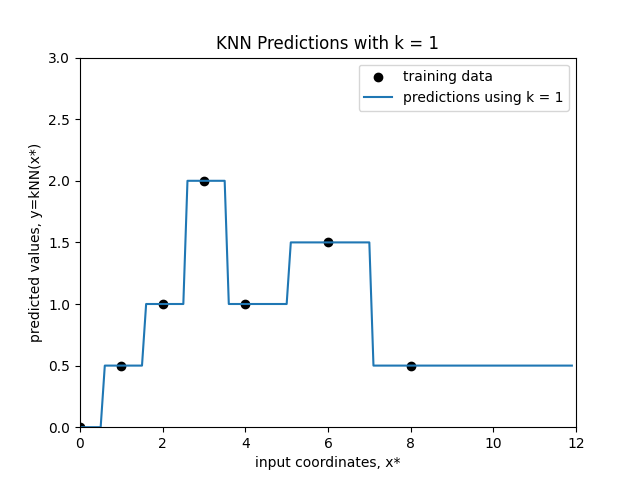
\includegraphics{k1.png}
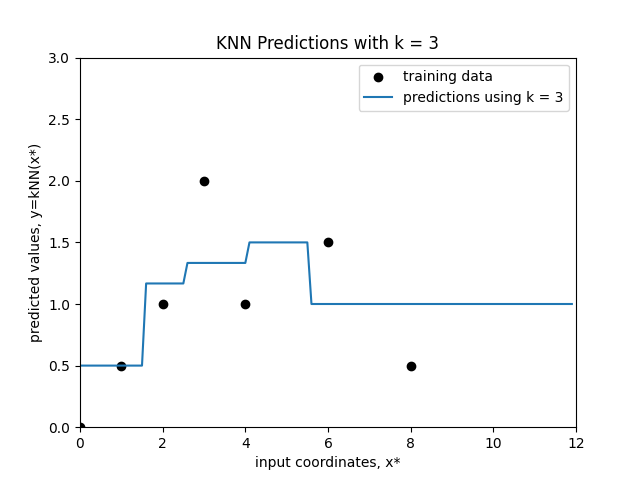
\includegraphics{k3.png}
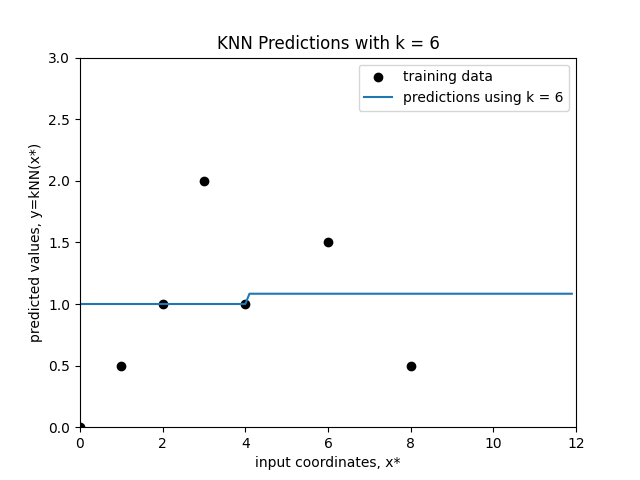
\includegraphics{k6.png}

  
  
\item k-NN with low k has some similar behavior to kernel-based regression with small lengthscale, while k-NN with high k has some similar behavior to kernel-based regression with large lengthscale.
  
  The 1-NN curve fits all the points exactly, as the previous kernel-based regression did when we set $\tau=0.01$. They also share the qualitative feature of jumping around a lot and being strongly influenced by nearby points to the extent that only the nearest training point affects a predicted y-value while all points farther away are disregarded. It has different behavior for interpolation in that x-values between but far from two training points will take on the y-value of one of those training points, unlike kernel-based regression with small lengthscale which predicted y-values of zero at most locations between the training points. The same effect is seen for x-values outside the range of the training data, where 1-NN simply extrapolates using the y-value of the first or last training point for every extreme x-value, whereas the kernel-based regression thinks that these x-values have very little similarity to the training data and therefore predicts a y-value of 0.
  
  The 3-NN curve has some similarity to the kernel-based regression with intermediate lengthscale, taking on values that represent some combination of the few nearest points.
  
  The 6-NN curve has the flattest slope, like the kernel-based regression with the longest lengthscale. This k-NN regressor basically uses something near the average y-value of most of the dataset and just predicts that value for every x-coordinate (with a small change near the middle of the x-range when the 7th point becomes closer than the 1st point).
  
  I do not think there are any values $k$ and $\tau$ such that the k-NN and kernel-based regressor would produce the same results for all x-coordinates. This is because the k-NN regressors extrapolate constant y-values when outside the x-values of the training data, while kernel-based predictions decay as the distance from the training points increases.
  
\item The choice of $\tau$ should not matter in the k-NN regressions, because no matter what value it is set to (as long as it is positive), it does not change the relative ordering of closeness kernel values, and we are only concerned with picking the $k$ closest points. Increasing $\tau$ by $1$ would divide all the kernel values by a factor of $e$ but would not change the ratios between them or their relative ranks.

\end{enumerate}

\newpage 

%%%%%%%%%%%%%%%%%%%%%%%%%%%%%%%%%%%%%%%%%%%%%
% Problem 3
%%%%%%%%%%%%%%%%%%%%%%%%%%%%%%%%%%%%%%%%%%%%%

\begin{problem}[Deriving Linear Regression, 10pts]

  The solution for the least squares linear regressions ``looks'' kind
  of like a ratio of covariance and variance terms.  In this problem,
  we will make that connection more explicit. \\

  \noindent Let us assume that our data are tuples of scalars $(x,y)$ that are
  described by some joint distribution $p(x,y)$.  For clarification, the joint distribution $p(x,y)$ is just another way of saying the ``joint PDF'' $f(x,y)$, which may be more familiar to those who have taken Stat 110, or equivalent. \\
  
  \noindent We will consider the process of fitting these data from this distribution with the best linear model
  possible, that is a linear model of the form $\hat{y} = wx$ that
  minimizes the expected squared loss $E_{x,y}[ ( y - \hat{y} )^2
  ]$.\\

\noindent \emph{Notes:} The notation $E_{x, y}$ indicates an
expectation taken over the joint distribution $p(x,y)$.  Since $x$ and
$y$ are scalars, $w$ is also a scalar.
  
  \begin{enumerate}

  \item Derive an expression for the optimal $w$, that is, the $w$
    that minimizes the expected squared loss above.  You should leave
    your answer in terms of moments of the distribution, e.g. terms
    like $E_x[x]$, $E_x[x^2]$, $E_y[y]$, $E_y[y^2]$, $E_{x,y}[xy]$
    etc.

\item Provide unbiased and consistent formulas to estimate $E_{x, y}[yx]$
 and $E_x[x^2]$ given observed data $\{(x_n,y_n)\}_{n=1}^N$.

\item In general, moment terms like $E_{x, y}[yx]$, $E_{x, y}[x^2]$,
  $E_{x, y}[yx^3]$, $E_{x, y}[\frac{x}{y}]$, etc. can easily be
  estimated from the data (like you did above).  If you substitute in
  these empirical moments, how does your expression for the optimal
  $w^*$ in this problem compare with the optimal $w^*$ that we see in
  Section 2.6 of the cs181-textbook?
  

\item Many common probabilistic linear regression models assume that
  variables x and y are jointly Gaussian.  Did any of your above
  derivations rely on the assumption that x and y are jointly
  Gaussian?  Why or why not?
    
\end{enumerate}

\end{problem}

\begin{enumerate}
    \item
    
    $$\mcL(w) = E\left[(y_n - \hat{y}_n)^2\right]$$
    
    $$\mcL(w) = E\left[y_n^2 - 2y_n\hat{y}_n + \hat{y}_n^2\right]$$
    
    $$\mcL(w) = E\left[y_n^2 - 2y_n w x_n + w^2 x_n^2\right]$$
    
    $$\mcL(w) = E[y_n^2] - 2 w E[x_n y_n] + w^2 E[x_n^2]$$
    
    $$ \frac{d\mcL}{dw} = 0 = -2E[x_n y_n] + 2w E[x_n^2]$$
    
    $$ E[x_n y_n] = w E[x_n^2] $$
    
    $$ w = E_{xy}[x y] / E_{x}[x^2] $$
    
    \item $$E_{x, y}[xy] = \frac{1}{N} \sum_{n=1}^{N} x_n y_n$$
    $$E_{x}[x^2] = \frac{1}{N} \sum_{n=1}^{N} x_n^2$$
    
    \item
    Substituting the formulas from 3.2 into the result of 3.1 gives the weight estimate:
  
  $$ w^* = \frac{E_{xy}[x y]}{E_{x}[x^2]} = \frac{\sum_{n=1}^{N} x_n y_n}{\sum_{n=1}^{N} x_n^2} $$
  
  The textbook gives the optimal weights (when $X$ has full column rank) as:
  
  $$ w^* = (X^T X)^{-1} X^T y $$
  
  which, when the $x$ and $y$ values are scalars, is equivalent to:
  
  $$ w^* = \frac{\sum \bold{x}\bold{y}}{\sum \bold{x}^2} $$
  
  summed across the list of all the values in $\bold{x}$ and $\bold{y}$. This is the same as the formula obtained by substituting the empirical moments into the result of 3.1.
  
  \item The formulas in 3.2 give unbiased estimates if x and y are jointly Gaussian but might produce biased or incorrect estimates for other possible joint distributions. In that sense, the formulas rely on the Gaussian distribution assumption. The derivation in 3.1 did not make any assumptions about the distributions of x and y.
 
 
\end{enumerate}


%%%%%%%%%%%%%%%%%%%%%%%%%%%%%%%%%%%%%%%%%%%%%
% Problem 4
%%%%%%%%%%%%%%%%%%%%%%%%%%%%%%%%%%%%%%%%%%%%%

\begin{problem}[Modeling Changes in Republicans and Sunspots, 15pts]
  
 The objective of this problem is to learn about linear regression
 with basis functions by modeling the number of Republicans in the
 Senate. The file \verb|data/year-sunspots-republicans.csv| contains the
 data you will use for this problem.  It has three columns.  The first
 one is an integer that indicates the year.  The second is the number
 of Sunspots observed in that year.  The third is the number of Republicans in the Senate for that year.
 The data file looks like this:
 \begin{csv}
Year,Sunspot_Count,Republican_Count
1960,112.3,36
1962,37.6,34
1964,10.2,32
1966,47.0,36
\end{csv}

You can see scatterplots of the data in the figures below.  The horizontal axis is the Year, and the vertical axis is the Number of Republicans and the Number of Sunspots, respectively.

\begin{center}
\includegraphics[width=.5\textwidth]{data/year-republicans}
\end{center}

\begin{center}
\includegraphics[width=.5\textwidth]{data/year-sunspots}
\end{center}

(Data Source: \url{http://www.realclimate.org/data/senators_sunspots.txt})\\
\vspace{-5mm}


\vspace{0.5cm}
\noindent\emph{Make sure to include all required plots in your PDF.}

\begin{enumerate}

\item In this problem you will implement ordinary least squares
  regression using 4 different basis functions for \textbf{Year
    (x-axis)} v. \textbf{Number of Republicans in the Senate
    (y-axis)}. Some starter Python code that implements simple linear
  regression is provided in \verb|T1_P4.py|.

  Note: The numbers in the \emph{Year} column are large (between $1960$ and $2006$), especially when raised to various powers. To avoid numerical instability due to ill-conditioned matrices in most numerical computing systems, we will scale the data first: specifically, we will scale all ``year'' inputs by subtracting $1960$ and then dividing by $40$. Similarly, to avoid numerical instability with numbers in the \emph{Sunspot\_Count} column, we will also scale the data first by dividing all ``sunspot count'' inputs by $20$. Both of these scaling procedures have already been implemented in lines $65-69$ of the starter code in \verb|T1_P4.py|. Please do \emph{not} change these lines!

First, plot the data and regression lines for each of the following sets of basis functions, and include
the generated plot as an image in your submission PDF. You will therefore make 4 total plots:
\begin{enumerate}
	\item[(a)] $\phi_j(x) = x^j$ for $j=1, \ldots, 5$\\
    ie, use basis $y = a_1 x^1 + a_2 x^2 + a_3 x^3 + a_4 x^4 + a_5 x^5$ for some constants $\{a_1, ..., a_5\}$. 
    \item[(b)] $\phi_j(x) = \exp{\frac{-(x-\mu_j)^2}{25}}$ for $\mu_j=1960, 1965, 1970, 1975, \ldots 2010$
	\item[(c)] $\phi_j(x) = \cos(x / j)$ for $j=1, \ldots, 5$
	\item[(d)] $\phi_j(x) = \cos(x / j)$ for $j=1, \ldots, 25$
\end{enumerate}
\vspace{-2mm}


{\footnotesize * Note: Please make sure to add a bias term for all your basis functions above in your implementation of the \verb|make_basis| function in \verb|T1_P4.py|.}
  
Second, for each plot include the residual sum of squares error. Submit the generated plot and residual sum-of-squares error for each basis in your LaTeX write-up.
\end{enumerate}

\end{problem}

\begin{framed}
\noindent\textbf{Problem 4} (cont.)\\
\begin{enumerate}
\setcounter{enumi}{1}
\item Repeat the same exact process as above but for \textbf{Number of Sunspots (x-axis)} v. \textbf{Number of Republicans in the Senate (y-axis)}. 
Now, however, only use data from before 1985, and only use basis functions (a), (c), and (d) -- ignore basis (b). You will therefore make 3 total plots. For each plot make sure to also include the residual sum of squares error.



Which of the three bases (a, c, d) provided the "best" fit? \textbf{Choose one}, and keep in mind the generalizability of the model. 

Given the quality of this fit, do you believe that the number of sunspots controls the number of Republicans in the senate (Yes or No)?
\end{enumerate}
\end{framed}

\begin{enumerate}
    \item
    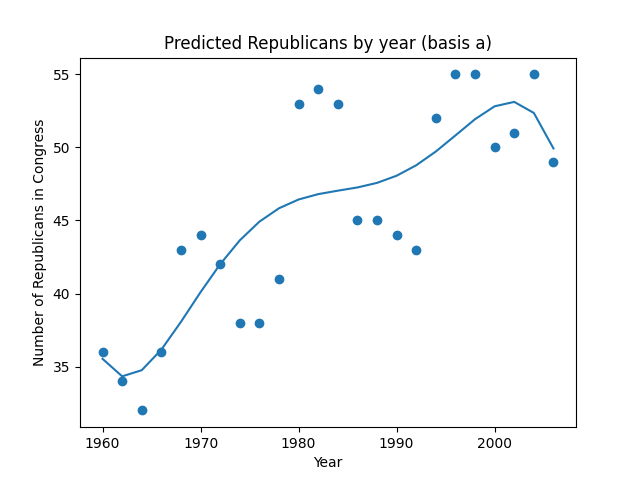
\includegraphics{41a.png}
    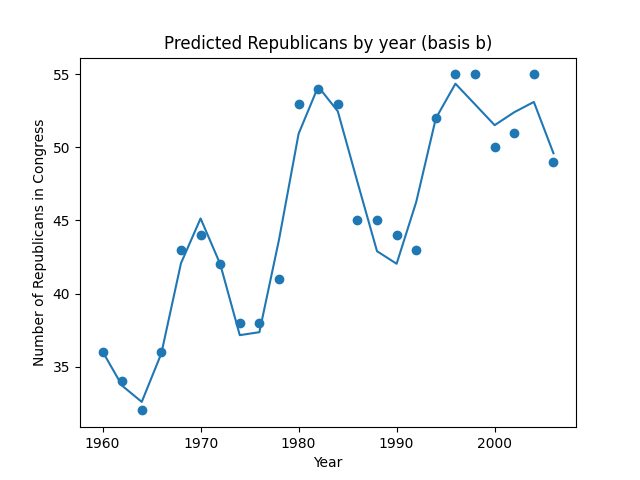
\includegraphics{41b.png}
    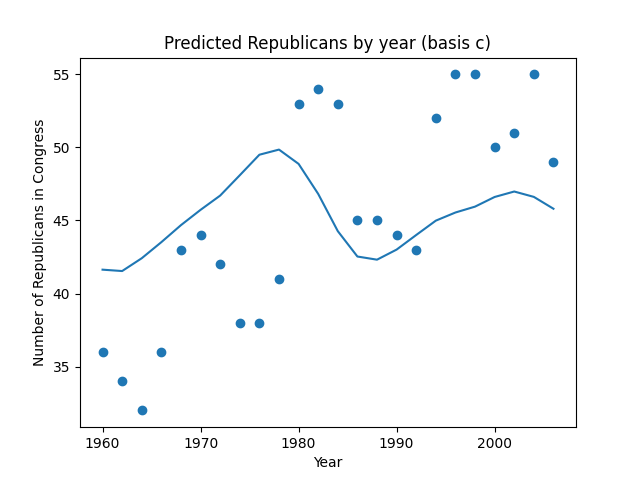
\includegraphics{41c.png}
    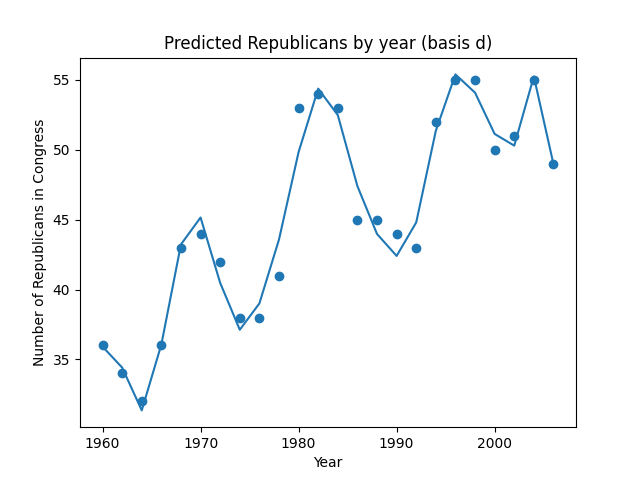
\includegraphics{41d.png}
    The total squared errors were:\\
    a. 394.98\\
    b. 54.27\\
    c. 1082.81\\
    d. 39.00\\
    \item
    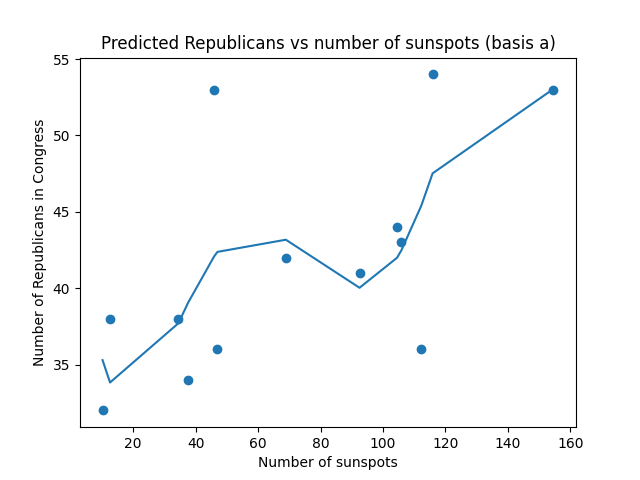
\includegraphics{42a.png}
    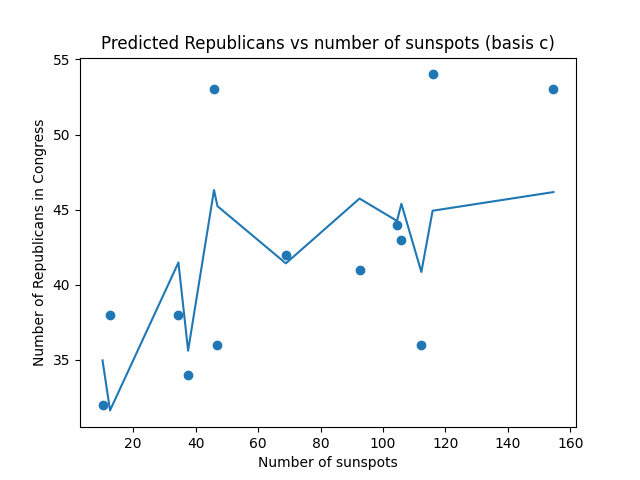
\includegraphics{42c.png}
    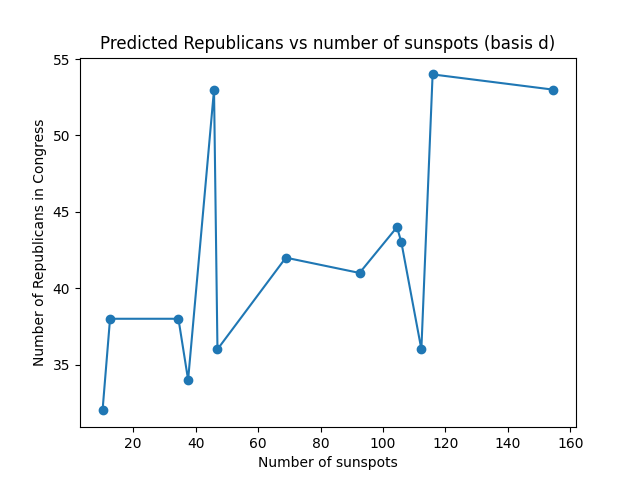
\includegraphics{42d.png}
    The total squared errors were:\\
    a. 351.23\\
    b. 375.11\\
    c. $4.9 \times 10^{-22}$\\
    Basis (d) provides the "best" fit in terms of least loss, but is extremely overfitted and would not generalize. Basis (a) might do better at interpolating for new values, so that is the one I would pick.
    However, I would not seriously attempt to use any of these bases or regression models to try to predict the number of Republicans in the Senate. Any correlation is probably spurious, and there is probably no relationship between sunspots and election outcomes.
\end{enumerate}



\newpage
%%%%%%%%%%%%%%%%%%%%%%%%%%%%%%%%%%%%%%%%%%%%%
% Name and Calibration
%%%%%%%%%%%%%%%%%%%%%%%%%%%%%%%%%%%%%%%%%%%%%
\subsection*{Name: Robi Rahman}

\subsection*{Collaborators and Resources}
Whom did you work with, and did you use any resources beyond cs181-textbook and your notes?

I gave some conceptual and programming assistance to Nikola Jurkovic. I did not use any resources besides the cs181-textbook and this PDF, which I read while studying regression using basis functions: http://www.cs.columbia.edu/~jebara/4771/tutorials/regression.pdf

\subsection*{Calibration}
Approximately how long did this homework take you to complete (in hours)?

20 hours

\end{document}